
%
%
% ISP
%
%
\subsection{Princípio da Segregação de Interface (Interface Segregation Principle - ISP)}
    
    \par O ISP orienta que os clientes de uma classe não devem ser forçados a depender de métodos que não utilizam. Este princípio promove a criação de interfaces menores, coesas e específicas para as necessidades de cada cliente, em detrimento de interfaces grandes e genéricas que tentam abranger múltiplas funcionalidades. O objetivo é evitar que classes implementem métodos desnecessários, o que pode levar a um acoplamento indesejado \cite{livro:martin:cleanarch}.

    \par A aplicação do ISP é importante para promover o desacoplamento, assegurando que as classes dependam apenas das interfaces que são estritamente relevantes para elas. Isso não apenas reduz o impacto de futuras alterações – já que uma mudança em uma interface específica afeta apenas os clientes que a utilizam – mas também torna a base de código mais flexível, modular e fácil de testar. Interfaces menores são mais fáceis de entender e implementar corretamente \cite{artigo:ramachandrappa:2024}.
    
    \par Um exemplo de violação do ISP, pode ser visualizado na Figura~\ref{fig:figura_isp_bad}.

    \begin{figure}[H]
        \centering
        
        \caption{Violação da ISP.}
        \label{fig:figura_isp_bad} 
        
        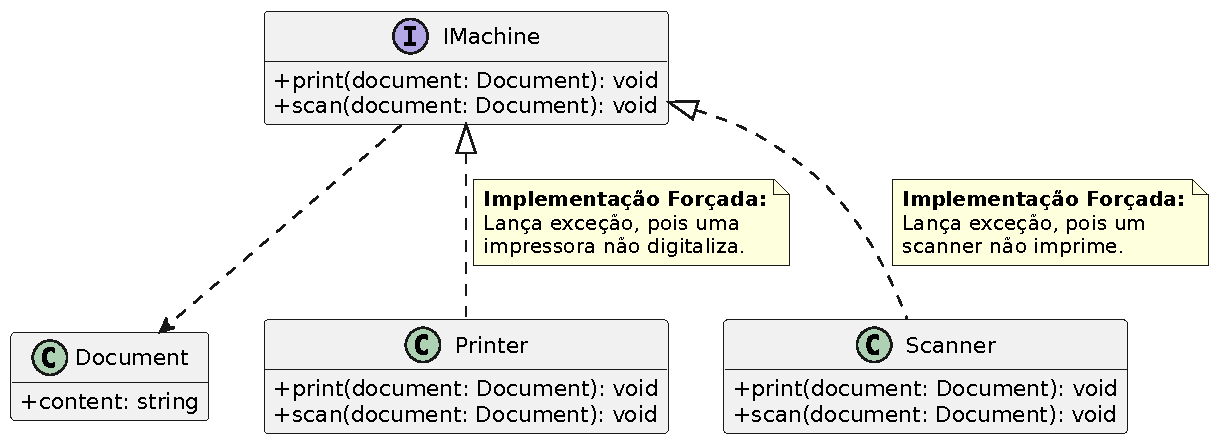
\includegraphics[width=1\linewidth]{figuras/solid/isp_bad.pdf}
        
        \fonte{Adaptado de \cite{artigo:ramachandrappa:2024}.}
    \end{figure} 
    
    \par Nesse caso tem-se uma interface IMachine que declara métodos print(Document document) e scan(Document document), as classes Printer e Scanner que implementam IMachine, forçando que as classes implementem métodos que não vão usar. Para aderir ao ISP, segue diagrama das interfaces segregadas na Figura \ref{fig:figura_isp_good}.
    
    \begin{figure}[H]
        \centering

        \caption{Aplicação da ISP.}
        \label{fig:figura_isp_good} 
        
        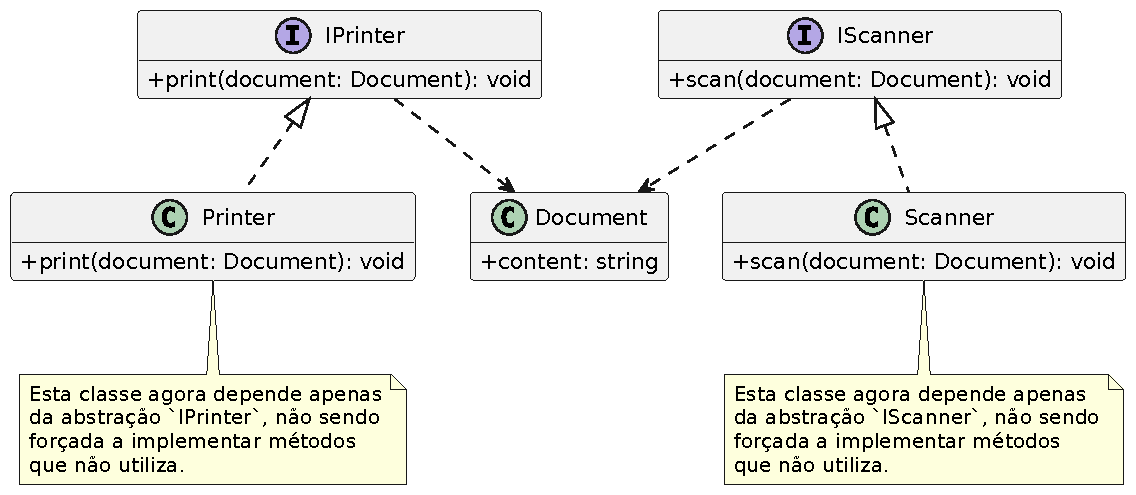
\includegraphics[width=1\linewidth]{figuras/solid/isp_good.pdf}
        
        \fonte{Adaptado de \cite{artigo:ramachandrappa:2024}.}
    \end{figure}
    
    \par Agora IMachine é dividida em interfaces mais granulares, como IPrinter e IScanner, permitindo que Printer implemente apenas IPrinter e Scanner implemente apenas IScanner, praticando a segregação das interfaces \cite{artigo:ramachandrappa:2024}.
        